\documentclass[UTF8,aspectratio=169,mathserif]{beamer}
\usepackage{ctex}
\usepackage{ulem}
\usepackage{color}
\usepackage{amssymb}
\usepackage{amsmath}
\usetheme{Berlin}
\setbeamertemplate{navigation symbols}{}

\title{5 - 多项式层级和交替}
\subtitle{The polynomial hierarchy and alternations}
\author{报告人:许博}
\date{\today}

\begin{document}
	
	\begin{frame}
		\titlepage
	\end{frame}
	
	\begin{frame}{目录}
		\tableofcontents
	\end{frame}
	
	\section{类 ${\bf\Sigma}_2^p$}
	\begin{frame}{似乎不能被 $\bf NP$-完全捕获的计算问题}
		\begin{block}{INDSET (NP-Complete)}
			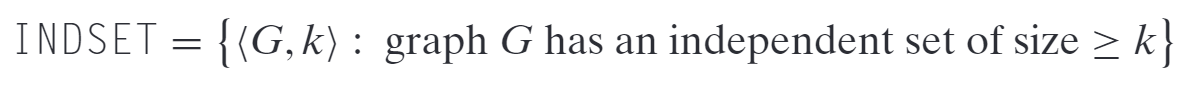
\includegraphics[width=0.6\linewidth]{../../5 & 6/note.assets/image-20210426152232421.png}
		\end{block}
		
		\begin{block}{EXACT INDSET}
			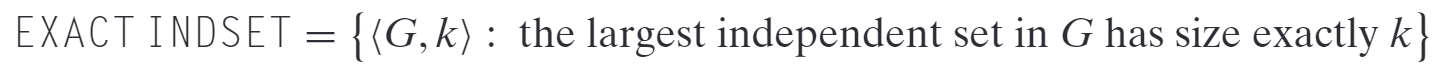
\includegraphics[width=0.7\linewidth]{../../5 & 6/note.assets/image-20210426152349887.png}
		\end{block}
		
		\begin{block}{MIN-EQ-DNF}
			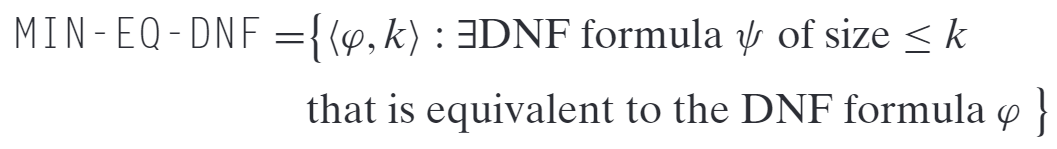
\includegraphics[width=0.6\linewidth]{../../5 & 6/note.assets/image-20210426152757453.png}
			
			其中 a DNF formula is a Boolean formula that is an OR of ANDs 
		\end{block}
	\end{frame}
	
	\begin{frame}{定义类 ${\bf\Sigma}_2^p$}
		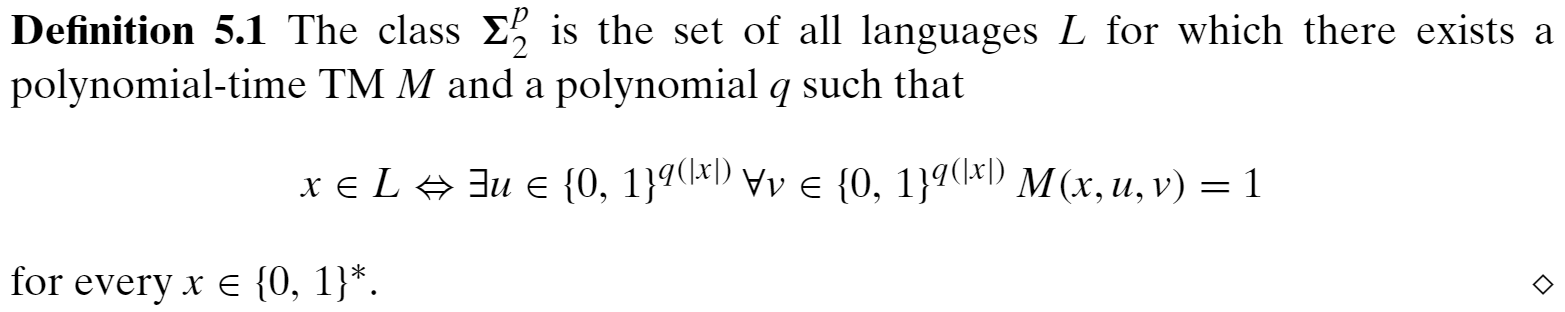
\includegraphics[width=\linewidth]{../../5 & 6/note.assets/image-20210426154842170.png}\newline
		
		1. ${\bf\Sigma}_2^p$ 包含(但不只包含)类 $\bf NP$ 和 $\bf coNP$;
		
		2. MIN-EQ-DNF 是 ${\bf\Sigma}_2^p$-完全问题。
	\end{frame}
	
	\section{多项式层级}
	\begin{frame}{$\bf PH$ 的定义}
		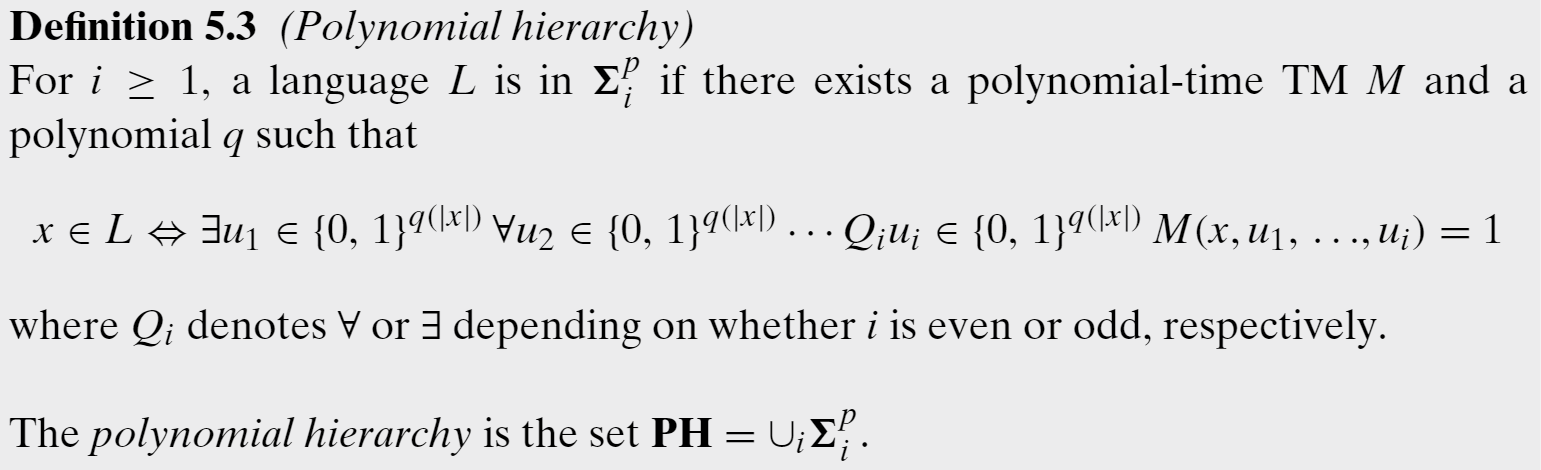
\includegraphics[width=\linewidth]{../../5 & 6/note.assets/image-20210426160324184.png}\newline
		
		定义 ${\bf\Pi}_i^p={\bf co\Sigma}_i^p=\{\overline{L}:L\in{\bf\Sigma}_i^p\}$。有 ${\bf\Sigma}_1^p={\bf NP}$。因此 ${{\bf\Pi}_1^p={\bf coNP}}$。
		
		并且有 ${\bf\Sigma}_i^p \subseteq{\bf\Pi}_{i+1}^p\subseteq{\bf\Sigma}_{i+2}^p$,因此${\bf PH}=\cup_{i>0}{\bf\Pi}_i^p$。
	\end{frame}
	
	\begin{frame}{$\bf PH$ 的性质}
		塌缩(collapse):如果存在 $i$ 使得 ${{\bf\Sigma}_i^p}={{\bf\Sigma}_{i+1}^p}$,则称 PH 塌缩,同时隐含 ${{\bf\Sigma}_i^p}={\cup}_{j\ge1}{{\bf\Sigma}_j^p}={\bf PH}$,这时可以说 PH 塌缩至第 $i$ 层。\newline
		
		“PH 不塌缩” 是 $\bf P\neq NP$ 以及 $\bf NP\neq coNP$ 猜想的一般形式。\newline
		
		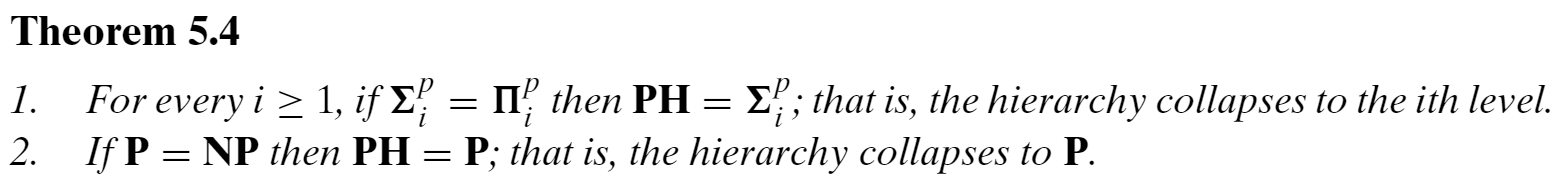
\includegraphics[width=\linewidth]{../../5 & 6/note.assets/image-20210427092228569.png}
	\end{frame}
	
	\begin{frame}{$\bf PH$ 不同层的完全问题}
		每个 $i\in\mathbb{N}$,${{\bf\Sigma}_i^p}$ 和 ${{\bf\Pi}_i^p}$ 都有完全问题,PH 没有完全问题(除非 PH 塌缩)\newline
		
		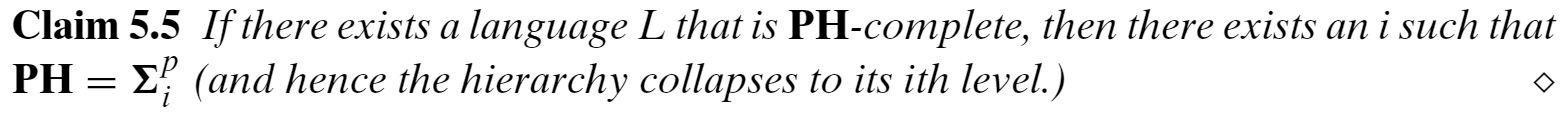
\includegraphics[width=\linewidth]{../../5 & 6/note.assets/image-20210427092442758.png}\newline
		
		如 $\bf NP$ 和 $\bf coNP$,$\bf PH$ 也包含于 $\bf PSPACE$。而除非 PH 塌缩,否则 $\bf PH\neq PSPACE$
	\end{frame}
	
	\begin{frame}
		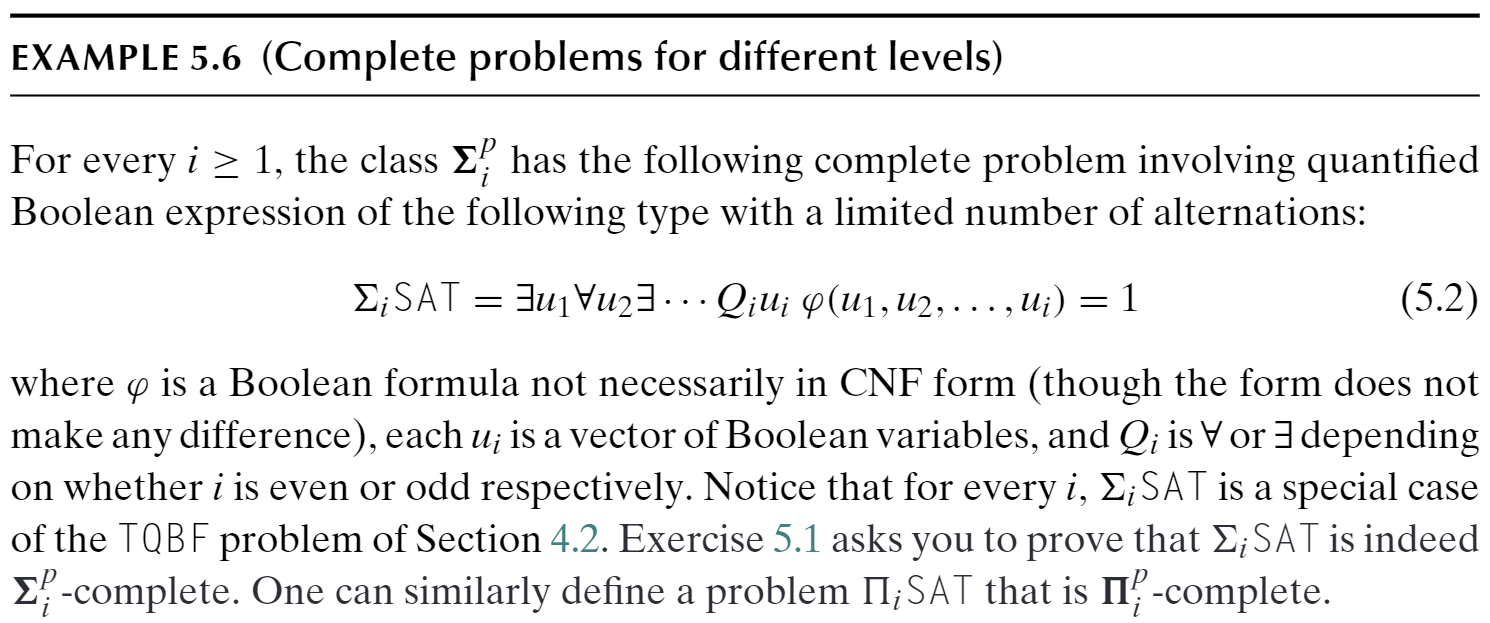
\includegraphics[width=\linewidth]{../../5 & 6/note.assets/image-20210427093527360.png}\newline
		
		需要注意的是,其中每个 $u_i$ 表示一组布尔变量。
	\end{frame}
	
	\section{交替图灵机}
	\begin{frame}{交替图灵机(Alternating TM)的定义}
		NDTM 不是一个现实的计算模型,但它有助于我们关注猜一个答案和验证它的区别。ATM 在没有明显的短证明的问题中起到类似的作用。\newline
		
		ATM 类似 NDTM,但其内部状态(除了接受和终止状态)会被 $\exists$ 或者 $\forall$ 标记。NDTM 接受输入当存在一条到达接受状态的路径时,可以看作每个内部状态都标记为 $\exists$,在 ATM 中,则可以在 $\exists$ 和 $\forall$ 之间交替选择。
	\end{frame}
	\begin{frame}
		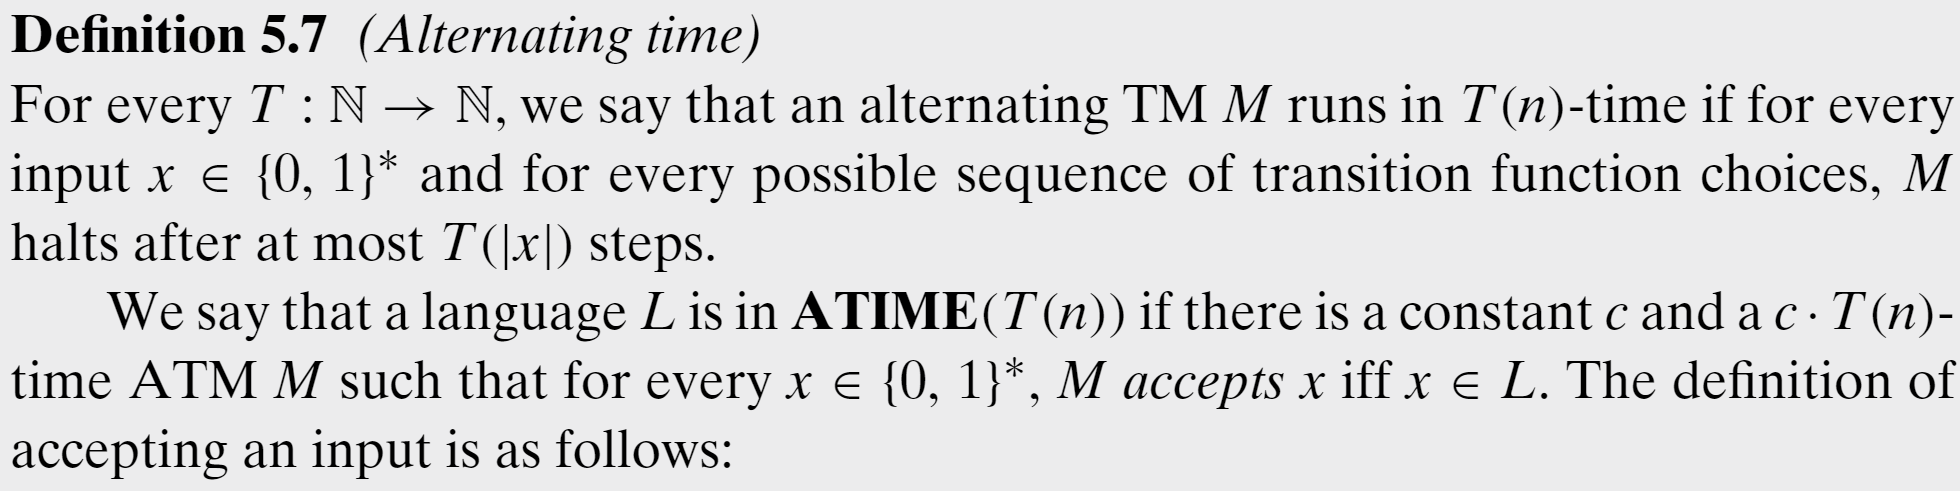
\includegraphics[width=\linewidth]{../../5 & 6/note.assets/image-20210427213236953.png}\newline
		
		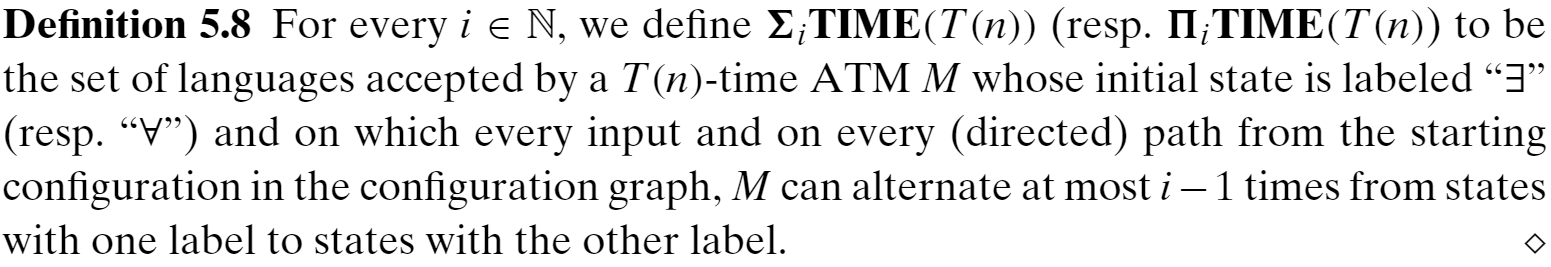
\includegraphics[width=\linewidth]{../../5 & 6/note.assets/image-20210427094554653.png}
	\end{frame}
	
	\begin{frame}{无限制的交替}
		PH 限制 ATM 中交替的个数取决于输入的大小,在移除这一限制后可以得到类 ${\bf AP}=\cup_c{\bf ATIME}(n^c)$,则有定理:\newline
		
		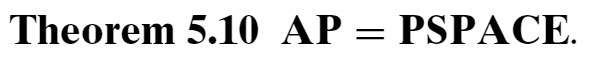
\includegraphics[width=0.4\linewidth]{../../5 & 6/note.assets/image-20210427095127253.png}\newline
		
		\begin{block}{TQBF}
			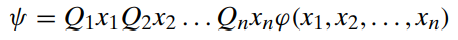
\includegraphics[width=0.5\linewidth]{../../5 & 6/note.assets/image-20210427225640198.png}
		\end{block}
	\end{frame}
	
	\section{通过预言机定义层级}
	\begin{frame}{通过预言机定义层级}
		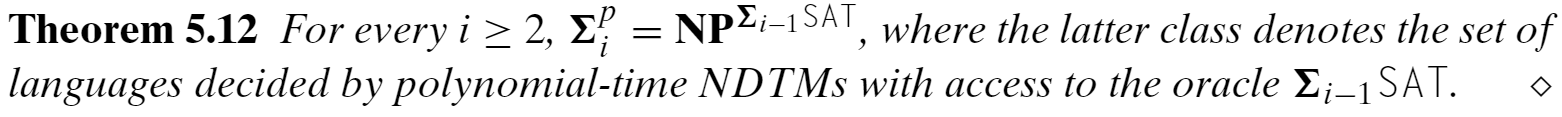
\includegraphics[width=\linewidth]{../../5 & 6/note.assets/image-20210427130304091.png}\newline
		
		1. 预言 SAT 的预言机也可以单步判定输入是否属于 SAT,因此也包括了判定 $\bf coNP$ 语言的能力。类似的,${\bf\Sigma}_i^p$ 是能够在解决 ${\bf\Sigma}_{i-1}^p$ 和 ${\bf co\Sigma}_{i-1}^p$ 的基础上(作为单位)的 $\bf NP$ 问题;\newline
		
		2. 因为一个类的完全问题的算法可以解决该类所有问题,可以用该类名替代对应的问题,比如表示 ${\bf\Sigma}_3^p$ 为 $\bf NP^{NP^{NP}}$。
	\end{frame}
	
	\section{SAT 的时间-空间权衡}
	\begin{frame}{SAT 的时间-空间权衡}
		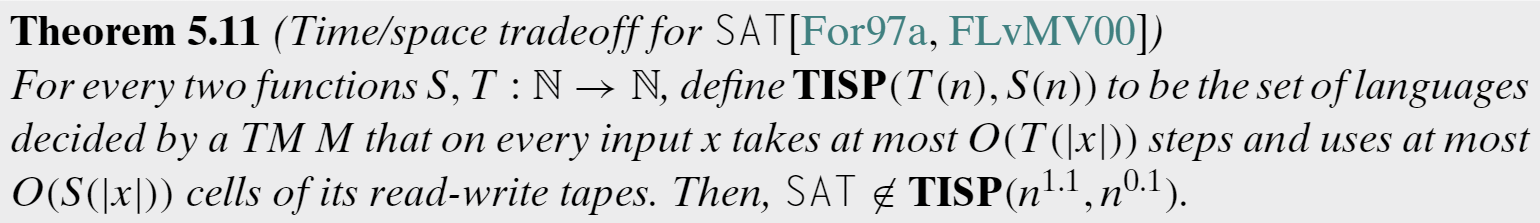
\includegraphics[width=\linewidth]{../../5 & 6/note.assets/image-20210427100533327.png}
	\end{frame}
	
\end{document}